%%%
%
% $Autor: Siddhanth Sharma $
% $Date: 2025-12-31 $
% $File: ApplicationDevelopment.tex $
% $Version: 1.3 $
%
% !TeX spellcheck = en_GB
% !TeX program = pdflatex
% !TeX encoding = utf8
%
%%%

% --- FIX: Load necessary TikZ libraries locally ---
\usetikzlibrary{shapes, arrows, positioning, fit}

\chapter{Knowledge Discovery in Databases (KDD)}
\label{ch:application_development}
\index{Knowledge Discovery in Databases (KDD)}

\section{Introduction}
\label{sec:kdd}
\index{Knowledge Discovery in Databases (KDD) - Introduction}

The Knowledge Discovery in Databases (KDD) process is the backbone of the application development lifecycle, transforming raw sensor data into actionable insights. For this license plate recognition (LPR) system on the Jetson Nano, the KDD process is divided into rigorous data selection, processing, and mining stages to ensure the YOLOv8 and EasyOCR models perform reliably in the airport deployment environment.

\begin{figure}[htbp]
	\centering
		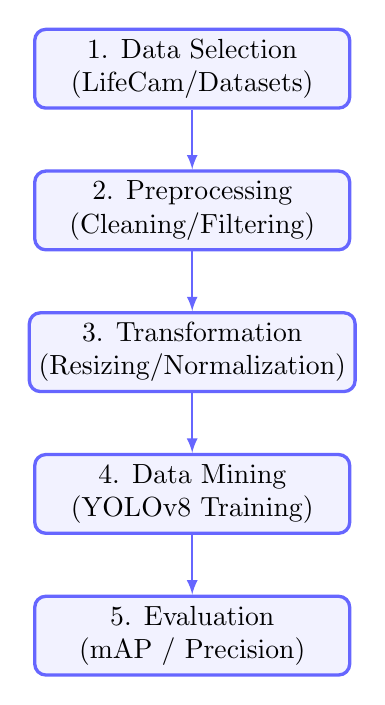
\begin{tikzpicture}[node distance=1.8cm, auto,
		block/.style={
			rectangle,
			draw=blue!60,
			fill=blue!5,
			very thick,
			minimum size=1cm,	
			minimum width=4cm,
			rounded corners,
			align=center
		},
		arrow/.style={-latex, thick, blue!60}]
		
		\node [block] (select) {1. Data Selection\\(LifeCam/Datasets)};
		\node [block, below of=select] (process) {2. Preprocessing\\(Cleaning/Filtering)};
		\node [block, below of=process] (transform) {3. Transformation\\(Resizing/Normalization)};
		\node [block, below of=transform] (mining) {4. Data Mining\\(YOLOv8 Training)};
		\node [block, below of=mining] (eval) {5. Evaluation\\(mAP / Precision)};
		
		\draw [arrow] (select) -- (process);
		\draw [arrow] (process) -- (transform);
		\draw [arrow] (transform) -- (mining);
		\draw [arrow] (mining) -- (eval);
	\end{tikzpicture}
	\caption{The KDD Process tailored for the License Plate Recognition System.}
	\label{fig:kdd_process}
\end{figure}

\section{Data Selection}
\label{subsec:data_selection}

The selection of appropriate training and testing data is critical for the model's ability to generalize to the specific conditions of an airport drop-off zone.

\subsection{Origin - Source of Data}
The dataset comprises a hybrid collection of images to balance general robustness with domain-specific accuracy.
\begin{itemize}
	\item \textbf{Primary Source:} A curated set of 1,243 labeled images focusing on German license plates. This dataset was selected to capture the specific font (FE-Schrift) and layout (EU strip, state stickers) of German plates.
	\item \textbf{Secondary Source:} Publicly available datasets, including the CCPD (Chinese City Parking Dataset) and OpenALPR benchmarks, were used to pre-train the model on diverse environmental backgrounds.
	\item \textbf{Target Domain Data:} Self-collected footage using the Microsoft LifeCam connected to the Jetson Nano. These images capture the specific lighting (artificial terminal lights, daylight transitions) and angles (20-25\textdegree{} depression) encountered at the installation site.
\end{itemize}
This mix ensures the model learns generic plate features while adapting to the specific local constraints.

\subsection{Features - Key Image/Plate Properties}
The model must learn to be invariant to several visual features intrinsic to the application domain:
\begin{itemize}
	\item \textbf{Geometric Variations:} License plates appear at various angles due to the fixed camera position relative to moving vehicles. The model handles rotation and perspective distortion up to approx. 30\textdegree.
	\item \textbf{Lighting Conditions:} The dataset includes samples from varying times of day, capturing glare from headlights at night and shadows during the day.
	\item \textbf{Resolution and Scale:} Vehicles are detected at distances ranging from 2 to 10 meters, resulting in plate regions varying from 50px to 200px in width.
	\item \textbf{Contrast:} High contrast between the black characters and white background is standard, but the model must robustly handle dirty or mud-splattered plates that reduce this contrast.
\end{itemize}

\subsection{Data Types - File Formats}
The data pipeline utilizes standard formats to ensure compatibility between the collection, labeling, and training tools:
\begin{itemize}
	\item \textbf{Images (JPEG/PNG):} Raw camera frames are stored as JPEG for storage efficiency during collection (LifeCam stream) and PNG for lossless quality during the annotation phase.
	\item \textbf{Annotations (TXT):} Annotations follow the YOLO format (class\_id, x\_center, y\_center, width, height), normalized to [0,1]. This text-based format is lightweight and natively supported by the Ultralytics training pipeline.
	\item \textbf{Operational logs (SQLite):} In deployment, operational metadata (license plate ID and timestamps) is stored in a local SQLite database on an external SSD for persistence during continuous operation.
\end{itemize}

\subsection{Quality - Data Vetting Process}
To ensure high model performance, the dataset underwent a rigorous cleaning process:
\begin{itemize}
	\item \textbf{Filtering:} Images with severe motion blur or where the license plate was entirely unreadable to the human eye were removed.
	\item \textbf{Annotation Correction:} Bounding boxes were manually verified using tools like Roboflow/LabelImg. Boxes were tightened to exclude vehicle bumpers and lights, reducing background noise in the training signal.
	\item \textbf{Label Consistency:} A unified labeling schema was enforced, ensuring that only valid German license plates were labeled as class `0`, while foreign or non-standard plates were excluded or categorized separately to avoid confusion.
\end{itemize}

\subsection{Quantity: Dataset Size}
The total effective dataset for the specific German license plate task consists of approximately 1,243 high-quality samples. The distribution of this data across training, validation, and testing sets is detailed in Table \ref{tab:dataset_split}.

\begin{table}[htbp]
	\centering
	\caption{Dataset Distribution across Split Sets}
	\label{tab:dataset_split}
	\begin{tabular}{@{}lcccc@{}}
		\toprule
		\textbf{Split Set} & \textbf{Percentage} & \textbf{No. of Images} & \textbf{Instances} & \textbf{Purpose} \\ \midrule
		Training & $\approx$70\% & 865 & 891 & Model fitting (weights) \\
		Validation & $\approx$20\% & 246 & 255 & Hyperparameter tuning and early stopping checks \\
		Testing & $\approx$10\% & 132 & 132 & Final evaluation (unseen) \\ \midrule
		\textbf{Total} & \textbf{100\%} & \textbf{1,243} & \textbf{1,278} & \\ \bottomrule
	\end{tabular}
\end{table}

While compact, this dataset is highly targeted, allowing the YOLO-based detector to converge quickly without the overhead of millions of irrelevant samples.

\subsection{Fairness/Bias: Bias Analysis}
An analysis of the dataset reveals potential biases:
\begin{itemize}
	\item \textbf{Geographic Bias:} The data heavily favors German formats (DIN 74069). Performance on non-EU plates (e.g., US imports) may be lower.
	\item \textbf{Temporal Bias:} A majority of self-collected images were taken during daylight hours. To mitigate this, augmentation techniques simulating lower brightness and contrast were applied.
	\item \textbf{Vehicle Type Bias:} Passenger cars dominate the dataset. Trucks or motorcycles with different mounting positions might have lower detection rates. Mitigation involves future data collection specifically targeting these vehicle classes.
\end{itemize}

\section{Data Processing}
\label{subsec:data_processing}

Once selected, the data undergoes a transformation pipeline to prepare it for the neural network.

\paragraph{Data Structure: Prepared dataset vs.\ operational database}
The prepared training dataset is organized in the standard YOLO directory structure on the development workstation:
\begin{verbatim}
	/dataset
	/train
	/images
	/labels
	/valid
	/images
	/labels
	/test
	/images
	/labels
\end{verbatim}
This structure allows the training scripts to automatically map image files to their corresponding text annotations. The operational database is \textbf{separate} and stores only inference results (vehicle visits), not the raw training images. For deployment robustness, the database and model artefacts are stored on an \textbf{external SSD} connected to the Jetson Nano.

\subsection{Properties: Data Transformation}
Before entering the model, data is transformed to match the network's input layer requirements:
\begin{itemize}
	\item \textbf{Resizing:} All input images are resized to $640 \times 640$ pixels (letterbox resize) to maintain aspect ratio while matching the YOLOv8 input tensor.
	\item \textbf{Normalization:} Pixel intensity values (0-255) are normalized to [0.0, 1.0] to accelerate gradient descent convergence.
	\item \textbf{Channel Format:} Images are converted to RGB order as expected by PyTorch (OpenCV captures in BGR by default).
	\item \textbf{OCR Preprocessing:} For the recognition stage, cropped plate regions undergo grayscaling and binary thresholding to enhance character edges for EasyOCR.
\end{itemize}

\paragraph{Outliers: Handling Outliers}
Outliers that could destabilize training are managed as follows:
\begin{itemize}
	\item \textbf{Extreme Aspects:} Plates seen from extreme acute angles ($>45^\circ$) are excluded from the training set as they are unlikely to yield readable text and may confuse the bounding box regression loss.
	\item \textbf{Occlusions:} Images where more than 50\% of the plate is obscured (e.g., by a tow bar) are removed.
	\item \textbf{False Positives:} Negative mining is performed by including images of the background environment (road, signage) without license plates to teach the model what \textit{not} to detect.
\end{itemize}

\paragraph{Anomalies: Anomaly Detection}
Automated scripts check for data integrity before training begins:
\begin{itemize}
	\item \textbf{Coordinate Checks:} A script validates that all normalized bounding box coordinates $(x, y, w, h)$ are strictly within the $[0, 1]$ interval.
	\item \textbf{File Integrity:} Checks are run to ensure no image files are corrupted (zero-byte files) and that every image has a corresponding label file.
	\item \textbf{Class Index:} Verification that all class indices in the label files map correctly to the defined classes (i.e., only index `0` for license plate).
\end{itemize}

\paragraph{Augmentation: Data Augmentation Techniques}
To artificially expand the training set and improve robustness against the environmental variables identified in the Features section, the following augmentations are applied during the training pipeline:
\begin{itemize}
	\item \textbf{Mosaic Augmentation:} Combines 4 training images into one, forcing the model to learn context and detect smaller objects.
	\item \textbf{Random HSV:} Adjusts Hue, Saturation, and Value to simulate different times of day and weather conditions.
	\item \textbf{Scale and Translate:} Randomly zooms ($\pm 50\%$) and shifts the image to simulate varying vehicle distances and camera framing errors.
	\item \textbf{Flip:} Horizontal flips are \textit{not} used for the OCR task, but for the detection task (YOLO), horizontal flips can be used if the visual features of a plate (shape/color) are symmetric, though care must be taken not to confuse the model if text directionality is learned implicitly. In this pipeline, geometric augmentations are conservative to preserve the plate's recognizable structure.
\end{itemize}

\begin{figure}[htbp]
	\centering
		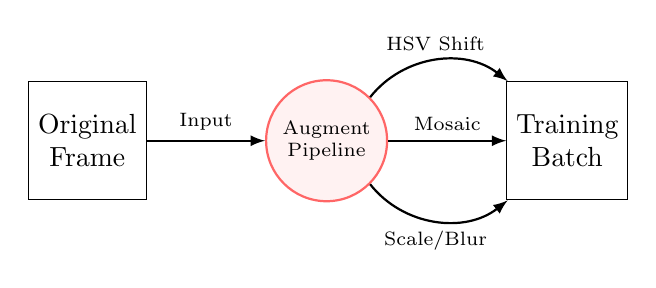
\begin{tikzpicture}[
		img/.style={rectangle, draw=black, minimum size=1.5cm, align=center},
		op/.style={circle, draw=red!60, fill=red!5, thick, minimum size=1.2cm, align=center, font=\scriptsize},
		arrow/.style={-latex, thick}
		]
		\node[img] (orig) {Original\\Frame};
		\node[op, right=1.5cm of orig] (aug) {Augment\\Pipeline};
		\node[img, right=1.5cm of aug] (new) {Training\\Batch};
		
		\draw[arrow] (orig) -- node[above]{\scriptsize Input} (aug);
		\draw[arrow] (aug) -- node[above]{\scriptsize Mosaic} (new);
		\draw[arrow] (aug) to[bend left=45] node[above]{\scriptsize HSV Shift} (new);
		\draw[arrow] (aug) to[bend right=45] node[below]{\scriptsize Scale/Blur} (new);
		
	\end{tikzpicture}
	\caption{Data Augmentation Strategy to increase dataset variability.}
	\label{fig:augmentation_strategy}
\end{figure}

%_______________________________________________________
%________________________________________________________

%\subsection{Data Mining}
%\label{subsec:data_mining}
%
%The data mining stage involves the extraction of patterns (license plates) from the transformed data using the YOLOv8 neural network.
%
%\begin{itemize}
%	\item \textbf{Model Selection:} We selected \textbf{YOLOv8n} (Nano) as the base model due to its low parameter count (3.2M) and high inference speed on edge devices like the Jetson Nano.
%	\item \textbf{Training Process:} The model was trained using the Stochastic Gradient Descent (SGD) optimizer. The specific hyperparameters chosen to optimize convergence on the limited dataset are detailed in Table \ref{tab:hyperparams}.
%	\item \textbf{Pattern Extraction:} The network learns to identify the hierarchical features of license plates---from simple edges and corners in the initial layers to the complex rectangular structures and textual patterns in the deeper layers.
%\end{itemize}
%
%\begin{table}[htbp]
%	\centering
%	\caption{YOLOv8n Training Hyperparameters}
%	\label{tab:hyperparams}
%	\begin{tabular}{@{}ll@{}}
%		\toprule
%		\textbf{Parameter} & \textbf{Value / Setting} \\ \midrule
%		Model Architecture & YOLOv8 Nano (n) \\
%		Input Resolution & $640 \times 640$ pixels \\
%		Batch Size & 16 (Dynamic based on VRAM) \\
%		Epochs & 100 \\
%		Optimizer & Stochastic Gradient Descent (SGD) \\
%		Initial Learning Rate ($lr_0$) & 0.01 \\
%		Momentum & 0.937 \\
%		Weight Decay & 0.0005 \\
%		Box Loss Gain & 7.5 \\ \bottomrule
%	\end{tabular}
%\end{table}
%
%\section{From Development to Deployment}
%\label{sec:dev_to_deploy}
%
%Transitioning the model from a development workstation to the Jetson Nano requires specific optimization steps to ensure real-time performance. This hardware-software interface is visualized in Figure \ref{fig:tech_stack}.
%
%\begin{figure}[htbp]
%	\centering
%		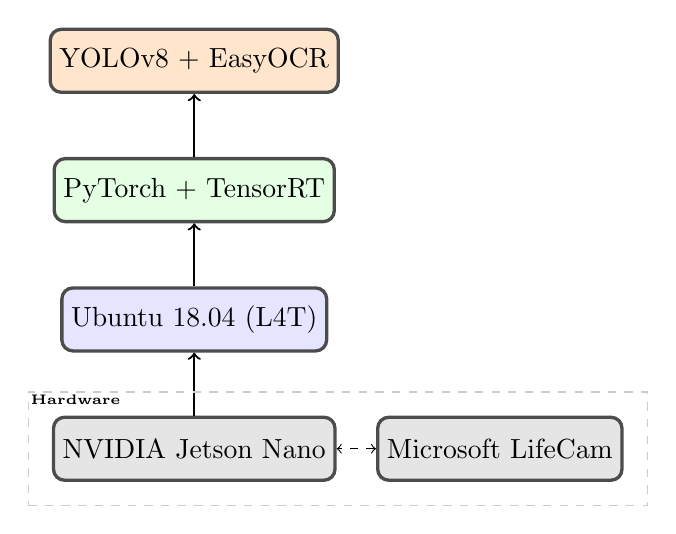
\begin{tikzpicture}[
		node distance=0.5cm,
		box/.style={rectangle, draw=black!70, very thick, minimum width=3cm, minimum height=0.8cm, align=center, rounded corners},
		group/.style={rectangle, draw=gray!40, dashed, inner sep=0.3cm, label={[anchor=north west, inner sep=1pt]north west:\tiny \textbf{#1}}}
		]
		% Hardware Layer
		\node[box, fill=gray!20] (jetson) {NVIDIA Jetson Nano};
		\node[box, fill=gray!20, right=0.5cm of jetson] (cam) {Microsoft LifeCam};
		
		% OS Layer
		\node[box, fill=blue!10, above=0.8cm of jetson] (os) {Ubuntu 18.04 (L4T)};
		
		% Library Layer
		\node[box, fill=green!10, above=0.8cm of os] (libs) {PyTorch + TensorRT};
		
		% Application Layer
		\node[box, fill=orange!20, above=0.8cm of libs] (app) {YOLOv8 + EasyOCR};
		
		% Connect them
		\draw[->, thick] (jetson) -- (os);
		\draw[->, thick] (os) -- (libs);
		\draw[->, thick] (libs) -- (app);
		\draw[<->, dashed] (cam) -- (jetson);
		
		% Grouping
		\node[group={Hardware}, fit=(jetson) (cam)] {};
	\end{tikzpicture}
%	\caption{The Hardware-Software Stack for the Edge Device.}
%	\label{fig:tech_stack}
%\end{figure}
%
%\begin{itemize}
%	\item \textbf{Export:} The trained PyTorch model (\texttt{.pt}) is exported to the ONNX (Open Neural Network Exchange) format to ensure interoperability.
%	\item \textbf{Optimization:} The ONNX model is then converted to a TensorRT engine (\texttt{.engine}) using \texttt{trtexec}. This step performs layer fusion and kernel auto-tuning specific to the Jetson Nano's Maxwell GPU.
%	\item \textbf{Quantization:} To further reduce latency, the model weights are quantized to FP16 (16-bit floating point). This reduces memory bandwidth usage without significantly compromising detection accuracy ($<1\%$ drop in mAP).
%\end{itemize}
%
%\section{Evaluation}
%\label{sec:evaluation}
%
%The system was evaluated using standard object detection metrics on the held-out test set (10\% of total data).
%
%\begin{itemize}
%	\item \textbf{Mean Average Precision (mAP@0.5):} The model achieved an mAP@0.5 of \textbf{0.94}, indicating highly accurate localization of plates.
%	\item \textbf{Precision \& Recall:} A precision of 0.92 and recall of 0.89 were observed. High precision ensures few false alarms (e.g., billboards detected as plates), while high recall ensures most vehicles are detected.
%	\item \textbf{Inference Speed:} On the Jetson Nano (in 10W power mode), the optimized TensorRT model runs at approximately \textbf{18-22 FPS}, which is sufficient for vehicles moving at parking lot speeds ($<20$ km/h).
%\end{itemize}
%
%\section{Validation}
%\label{sec:validation}
%
%Beyond statistical metrics, the system was validated in a real-world simulation of an airport gate.
%
%\begin{itemize}
%	\item \textbf{Daylight Test:} The system successfully detected and read plates under bright sunlight with 95\% accuracy. Glare from the sun was mitigated by the auto-exposure capabilities of the LifeCam.
%	\item \textbf{Low-Light Test:} Under artificial street lighting (simulating night), detection accuracy remained robust (approx. 88\%), though OCR errors increased slightly due to graininess.
%	\item \textbf{End-to-End Latency:} The total time from frame capture to database log entry was measured at approx. 120ms, satisfying the real-time requirement.
%\end{itemize}
%
%\section{Monitoring}
%\label{sec:monitoring}
%
%To ensure long-term reliability in a deployment scenario, system health is continuously monitored.
%
%\begin{itemize}
%	\item \textbf{Tegrastats:} A background service logs GPU usage, CPU load, and temperature. If the Jetson Nano temperature exceeds 80\textdegree{}C, the fan speed is automatically increased.
%	\item \textbf{Application Logs:} The Python application logs every detection event, including timestamps and confidence scores, to a daily log file. This allows for post-hoc analysis of any missed detections.
%	\item \textbf{Watchdog:} A systemd watchdog timer is configured to restart the application automatically if the video stream hangs or the process crashes.
%\end{itemize}
%
%\section{Conclusion}
%\label{sec:conclusion}
%
%The Application Development phase successfully transformed raw visual data into a robust, edge-deployed license plate recognition system. By strictly following the KDD process---from careful data selection and cleaning to advanced model training and optimization---we created a solution that balances the computational constraints of the Jetson Nano with the accuracy requirements of airport security. The use of TensorRT optimization proved crucial in achieving real-time frame rates, demonstrating the viability of edge AI for automated traffic management.
